\documentclass[twoside,11pt]{article}

\usepackage{blindtext}

% Any additional packages needed should be included after jmlr2e.
% Note that jmlr2e.sty includes epsfig, amssymb, natbib and graphicx,
% and defines many common macros, such as 'proof' and 'example'.
%
% It also sets the bibliographystyle to plainnat; for more information on
% natbib citation styles, see the natbib documentation, a copy of which
% is archived at http://www.jmlr.org/format/natbib.pdf

% Available options for package jmlr2e are:
%
%   - abbrvbib : use abbrvnat for the bibliography style
%   - nohyperref : do not load the hyperref package
%   - preprint : remove JMLR specific information from the template,
%         useful for example for posting to preprint servers.
%
% Example of using the package with custom options:
%
% \usepackage[abbrvbib, preprint]{jmlr2e}

\usepackage{jmlr2e}

\usepackage{mathtools}
\usepackage{amsmath}  % use argmin + argmax, cf. https://tex.stackexchange.com/a/5255
\DeclareMathOperator*{\argmax}{arg\,max}
\DeclareMathOperator*{\argmin}{arg\,min}
\usepackage{bm}

\usepackage{enumitem}  % nested enumerations, cf. https://tex.stackexchange.com/a/126756

% Definitions of handy macros can go here

\newcommand{\dataset}{{\cal D}}
\newcommand{\fracpartial}[2]{\frac{\partial #1}{\partial  #2}}

% Heading arguments are {volume}{year}{pages}{date submitted}{date published}{paper id}{author-full-names}

\usepackage{lastpage}
\tabmlheading{WS 2024/25}{1-\pageref{LastPage}}{15.03.2025}{}{Simon Stürzebecher}

% Short headings should be running head and authors last names

\ShortHeadings{Interpretable Neural Networks using EAGGA}{Simon Stürzebecher}
\firstpageno{1}

\begin{document}

\title{Interpretable Neural Networks using EAGGA}

\author{\name Simon Stürzebecher \email simon.stuerzebecher@campus.lmu.de}

%\editor{My editor}

\maketitle

\begin{abstract}%   <- trailing '%' for backward compatibility of .sty file
%\blindtext
- tabular data still difficult for NNs, where it's still outperformed by other ML model classes
- research suggests NN performance benefits from heavy regularisation
- using EAGGA, we regularise an NN and achieve both comparable performance as XGB on EAGGA as well as interpretability
- for this, we propose a network architecture specifically suited for the EAGGA algorithm
\end{abstract}

\begin{keywords}
  tabular data, multi-objective optimization, interpretability, deep learning
\end{keywords}

\section{Introduction}
Tabular Data
- most common type of data
- still difficult for neural networks
- \citep[p. 7499]{Borisov_2024}
- recent research suggests that strong regularisation is beneficial to NN performance on tab data \citep[8]{NEURIPS2021_c902b497}

- we know regularisation from linear models can come with improvements in interpretabiltiy
  * e.g. LM-LASSO (L1) regularisation as feature selection -> reduces \# features used in model by setting some coeffs to 0 \citep[p. 267]{lasso}
- other forms of regularisation improve performance
  * e.g. LM-Ridge (L2) on multi-collinear data \citep[p. 55]{ridge}  % TODO: mention in "extension" section that L2 is implemented via weight decay
  * e.g. NN dropout, reduces co-adaptation \citep[p. 1]{hinton2012improvingneuralnetworkspreventing}
  * e.g. NN early stopping, reduces overfitting on training data \citep[p. 778f]{early_stopping}

- we want to explore if we can use NN regularisation to tackle both interpretability and improved performance (i.e. ``comparable'' to XGBoost) on tab data
- using EAGGA framework, which proved it can improve performance while keeping (already high) performance of XGBoost on tab data -> see if interpretabiltiy
  improvements translate to NN + performance can also be on par


%\blindmathpaper


\section{Background and Related Works}

\subsection{Interpretability}
As there is no clear definition for interpretability, we will consider it as ``the ability to provide \textit{explanations} in \textit{understandable terms} to a human'',
where \textit{explanations} are logical decision rules and \textit{understandable terms} relate to commonly used terms in the domain of the problem,
as suggested by \citet[chap. 1]{survey_NN_interpretability}. Further, we use the term ``explainability'' in an exchangeable manner with ``interpretability'',
as is commonly done.

% Why Interpretability is desirable?
Explainability of a model's reasoning is in many ways desirable. \citet[pp. 3-4]{Zach2019InterpretabilityOD} gives a range of examples,
amongst which are \textit{gaining trust}, e.g. when doctors rely on medical diagnosis predictions, avoiding \textit{subconcious biases} by
making sure loan approvals are non-discriminatory, or \textit{regulatory} reasons, most notably the EU's ``Right to Explanation'' warranted by the
GDPR \citep[p. 1]{review_NN_interpretability} or for approval of drugs discovered using machine learning models \citep[1B]{survey_NN_interpretability}.
It can further prove helpful for explaining unexpected drops in model performance, which could arise from optimising a model with respect to loss and then judging its
performance on a different metric such as accuracy, a practice known as \textit{model debugging} \citep[1B]{survey_NN_interpretability} or for
\textit{scientific understanding} in domains where only models can make sense of increasingly complex data anymore and learnt knowledge encoded in a model needs to be
made accessible to humans to be used reliably \citep[p. 1]{review_NN_interpretability}.

Commonly, methods for model interpretation are divided into intrinsic methods, where the search space only comprises models with a structure simple enough to be
considered ``explainable'' (such as tree-based or simple linear models), and post-hoc methods, where interpretation methods are applied after model training.
Amongst post-hoc techniques, we can further divide the space into model-specific (such as analysing GLM coefficients) and model-agnostic
(e.g. partial depence plots, ALE) methods \citep[chap. 3.2]{molnar2022}.

% Taxonomy
\citet[chap. 2]{survey_NN_interpretability} extend this distinction to a three-dimensional taxonomy, allowing for better categorisation of neural networks (NNs),
a model class that in its fully-connected feedforwad form is inherently non-interpretable. % TODO: letztes halbsatz vllt lieber in intro unterbringen, hier ist der awkward und unnötig ausschmückend
\\
\textbf{Passive vs Active Approaches}, where \textit{passive} are all post-hoc methods and \textit{active} methods actively change either the architecture or
training process to increase model interpretability.
\\
\textbf{Type of Explanations}, distinguishing between \textit{example} methods, providing concrete examples of what leads to a desired output, \textit{attribution}
methods that attribute the effect on the output for a specific feature, \textit{hidden semantic} methods, which explain the types of inputs particular neurons or layers
pick up on, and logical \textit{rules}, such as if-then clauses or tree-induced rules.
\\
\textbf{Local vs Global Interpretability}, ranging from \textit{local} methods providing explanations based on individual samples, \textit{semi-local} methods,
explaining model behaviour for sets of samples grouped by some criterion, to \textit{global} methods, which explain the network as a whole.

% Evaluation
Given its unclear definition, evaluating interpretability can be challenging. \citet[3]{DoshiVelez2017TowardsAR} propose a taxonomy to categorise
possible evaluation methods based on their rigorousness.
\\
\textbf{Application-grounded evaluation} evaluates interpretations directly with respect to the task, by having human experts evaluate the outcome and
is therefore the most expensive and time-consuming of the three approaches.
\\
\textbf{Human-grounded metrics} is similar to application-grounded evaluation in that a human still evaluates the interpretations, but tries to simplify the task
so that a layperson can do it. Human-grounded approaches are especially suitable if it's sufficient to validate the general concepts of a task. A typical evaluation
set-up in this category is binary forced choice, where the human evaluator chooses, which of two generated explanations he prefers.
\\
\textbf{Functionally-grounded evaluation} is the least rigorous, but easiest to implement of the three. It assess explanatory quality according to some
formally defined proxy for interpretability and is particularly useful in ranking different models if their model-class is already identified
(e.g. via human-grounded evaluation) to be interpretable. The main challenge for functionally-grounded evaluation is finding a good proxy.

\subsection{Hyperparameter Optimization (HPO)}
In contrast to model parameters, which are optimized during training, hyperparameters (HPs) are those describing the machine learning algorithm and are
fixed before training. Because they usually have a significant impact on the trained model's performance, HPs are often optimized, too.
Let $\mathcal{D}\subseteq\mathcal{X}\times\mathcal{Y}$ be a dataset consisting of $n$
tuples drawn from the data-generating distribution, i.e. $(\boldsymbol{x}^{(i)}, y^{(i)})\stackrel{i.i.d.}{\sim}\mathbb{P}_{\boldsymbol{x}y},\forall i=1,...,n$.
Furthermore, let $\mathcal{I}:(\mathbb{D}\times\boldsymbol\Lambda)\rightarrow\mathcal{H}, (\mathcal{D},\boldsymbol\lambda)\mapsto\hat{f}$
be an algorithm that maps a given dataset $\mathcal{D}$ and HP configuration $\boldsymbol\lambda\in\boldsymbol\Lambda$ to a model $\hat{f}$.
Denote with $\mathcal{I}_{\boldsymbol\lambda}$ an algorithm with fixed HP configuration a chosen loss function with $L$.
The goal of model training is, for fixed $\boldsymbol\lambda$, to have $\mathcal{I}_{\boldsymbol\lambda}$ find model $\hat{f}$ minimising the expected generalisation error
$GE(\mathcal{I}_{\boldsymbol\lambda},\mathcal{D},L)=\mathbb{E}_{(\boldsymbol{x},y)\sim\mathbb{P}_{\boldsymbol{x}y}}[L(y,\mathcal{I}_{\boldsymbol\lambda}(\mathcal{D})(\boldsymbol{x}))]$
The goal of HPO, on the other hand, is to find $\boldsymbol\lambda$ minimising the expected generalisation error,
i.e. $\argmin_{\boldsymbol\lambda\in\boldsymbol\Lambda} GE(\mathcal{I}_{\boldsymbol\lambda},\mathcal{D},L)$.
For this, there is no analytical expression available, making HPO a blackbox optimization problem. \citep[pp. 2f]{10.1145/3610536}

We will first outline model-free methods to approach blackbox optimization problems, before presenting a model-based variant.

% model free
% grid + random search
The most basic model-free strategies for blackbox optimization are grid and random search.
In the latter, the user defines a range of interest for each HP and then evaluating points along a grid within the cartesian product of those.
This has the drawback of scaling extremely poorly in both number of HP dimensions and number of query points per range of interest.
Random search, on the other hand, randomly samples a value for each HP until it runs out of budget. Its explorative nature, ease of use, and no assumptions
about the model makes it a good baseline. It is also superior to grid search in cases were one or more HPs have little impact on model performance,
as for a given budget $B$, each HP will likely be queried with $B$ different values, whereas for grid search each HP will only be queried with $B^{1/N}$
different values for $N$ HPs. \citep[chap. 1.3]{feurer_hyperparameter_2019}

% evolutionary algorithms
Another popular class of model-free optimizers are evolutionary algorithms (EAs), which are conceptually simple and can handle even complex parameter spaces,
given appropriate implementation of operators.
EAs are iteratively evolving a population of individuals (an individual is simply a hyperparameter configuration) of size $\mu$, where in each iteration (generation),
$\lambda$\footnote{We distinguish between $\lambda\in\mathbb{N}$ when referring to the offspring size of EAs and $\boldsymbol\lambda\in\boldsymbol\Lambda$ when
referring to a hyperparameter configuration.} offspring are generated via three operators \citep[pp. 10-14]{genetic_algos}.
\\
\textbf{Reproduction} samples an individual from the population to reproduce with probability proportional to its fitnes. For HPO, fitness usually refers to the
performance metric the model resulting from the individual's HP configuration is evaluated on.
\\
\textbf{Crossover} selects two ``parents'' from the pool of reproducing individuals. An index $k$ is sampled at random and all HP values from
index $k$ on are swapped, yielding two new ``children'' individuals.
\\
\textbf{Mutation} randomly changes single HP values of an individual chosen for reproduction, e.g. by adding Gaussian noise to real values or flipping bits
on binary values.
\\
At the end of each generation, the EA keeps the best $\mu$ individuals, either only from the offspring (``$(\mu,\lambda)$-selection'') or more commonly from
population and offspring (``$(\mu+\lambda)$-selection''), which is also called an ``elitist'' strategy, as it's guaranteed to keep the best individual.
\citep[chap. 1.3]{feurer_hyperparameter_2019}

One of the most popular EA implementations is the ``Covariance Matrix Adaptation Evolution Strategy'' (CMA-ES).
It employs a multivariate normal distribution to generate offspring, for which the mean is a weighted average of the previous generation's individuals
and the covariance matrix similarly is the weighted covariance of the previous generation.
The weighing scheme for both is done in a way as to reproduce previously successful (i.e. selected) steps \citep[p. 8-11]{hansen2023cmaevolutionstrategytutorial}.

Another popular EA approach is Differential Evolution. Its populaton is randomly initialised so the entire search space is covered.
In each generation $g$, for each $\boldsymbol\lambda_{i,g}$ with $i=1,...,n$ it creates ``mutant vectors''
$\boldsymbol\nu_{i,g+1}=\boldsymbol\lambda_{r_1,g}+F\cdot(\boldsymbol\lambda_{r_2,g}-\boldsymbol\lambda_{r_3,g})$,
where $r_1,r_2,r_3\in\{1,...,n\}$ are mutually different random indices that also different from $i$ and $F\in[0,2]$ is constant.
For crossover, it then generates a ``trial vector'' $\boldsymbol\upsilon_{i,g+1}=(\upsilon_{i,g+1}^{(1)},\upsilon_{i,g+1}^{(2)},...,\upsilon_{i,g+1}^{(N)})^T$ with
\begin{equation}
  \upsilon_{i,g+1}^{(j)} = \begin{dcases}
    \nu_{i,g+1}^{(j)} & \text{if } u\le\text{CR}\text{ or } j=R \\
    \lambda_{i,g}^{(j)} & \text{else}
  \end{dcases}
\end{equation}
for a random index $R\in\{1,2,...,D\}$, sampled $u\sim U[0,1]$, and crossover constant $\text{CR}\in[0,1]$.
Selection is done by picking the better of $\boldsymbol\upsilon_{i,g+1}$ and $\boldsymbol\lambda_{i,g}$ with respect to fitness. \citep[p. 343]{differential_evolution}

% model based
Contrasting to model-free approaches, model-based methods fit a surrogate model on the target function and optimize the surrogate.
Currently, one of the most popular model-based approaches is Bayesian Optimization (BO).
BO is an iterative algorithm comprising a probabilistic surrogate model $\tilde{f}$ for the blackbox problem $f$ and an acquisition function.
It maintains and continually extends a set of points it already evaluated on the target function.
In each iteration, the posterior predictive distribution is determined by fitting the surrogate model on this set of points.
The acquisition function then retrieves the highest utility point from the surrogate model and evaluates it on the target function, after which it adds the point
to the set of queried points \citep[chap. 1.3.2]{feurer_hyperparameter_2019} and \citep[pp. 2f]{frazier2018tutorialbayesianoptimization}.
Evidently, neither the target function nor the surrogate model are optimized directly. Rather, the acquisition function trades-off exploration and exploitation of
the surrogate and is maximised to yield the next query point most likely to optimize the two objectives as defined by the acquisition function.
\\
Common choices for the acquisition function are Expected Improvement (Eq. \ref{eq-expected-improvement}) and Thompson Sampling (Eq. \ref{eq-thompson-sampling}).
\begin{equation}
  \text{EI}_t(\boldsymbol\lambda):=\mathbb{E}_t[(f(\boldsymbol\lambda)-f_t^*)^+]
  \label{eq-expected-improvement}
\end{equation}
\textbf{Expected Improvement} computes the expected minimisation over the incumbent $f_t^*$ for evaluating the target function $f$ at query point $\boldsymbol\lambda$.
$\mathbb{E}_t$ denotes the expectation under the posterior predictive distribution with $t$ query points, similarly, the current incumbent is the minimum value
of the target function from previous evaluations $(\boldsymbol\lambda_{1:t},f(\boldsymbol\lambda_{1:t}))$. \citep[p. 7]{frazier2018tutorialbayesianoptimization}
\begin{equation}  % TODO: take out
  f^{(t)}\sim\tilde{f}_t
  \label{eq-thompson-sampling}
\end{equation}
\textbf{Thompson Sampling}, on the other hand, can conceptually be described as drawing a candidate function $f^{(t)}$ from the posterior predictive distribution and
minimising it to obtain the next query point for the target function. \citep[p. 161]{7352306}
\\
Composing the other part of BO, surrogate models need to be able to model mean and variance of its target function estimate.
Commonly chosen models are Gaussian Processes (Eq. \ref{eq-gaussian-process}) and Random Forests.
\begin{equation}  % TODO: make inline or provide further information
  \text{GP}(m(\boldsymbol\lambda), k(\boldsymbol\lambda,\boldsymbol\lambda'))
  \label{eq-gaussian-process}
\end{equation}
\textbf{Gaussian Processes} (GP) are fully specified by their mean and covariance functions and have closed-form solutions.
The mean $m(\boldsymbol\lambda)$ fits all points already evaluated on the target function, while for the covariance or
kernel function $k(\boldsymbol\lambda,\boldsymbol\lambda')$ it is desirable that points close to
each other in HP space $\boldsymbol\Lambda$ exhibit stronger correlation than those far apart.
The kernel function can be freely chosen, a common choices is the Gaussian (Eq. \ref{eq-kernel-gaussian}) kernel with
hyperparameter $\alpha_0$. \citep[p. 5]{frazier2018tutorialbayesianoptimization}
\begin{equation}
  k(\boldsymbol\lambda,\boldsymbol\lambda')=\alpha_0 \exp(-\|\boldsymbol\lambda-\boldsymbol\lambda'\|_2^2)
  \label{eq-kernel-gaussian}
\end{equation}
A drawback of Gaussian Processes is its poor scalability in number of data points and number of hyperparameters, although there exist workarounds approximating the full GP
with only a subset of the samples. \citep[chap. 1.3.2]{feurer_hyperparameter_2019}
\\
\textbf{Random Forests}, unlike GPs, can handle complex hyperparameter spaces even including categorical and hierarchical HPs. Their computational complexity is also far
less, making them a popular alternative to Gaussian Processes. \citep[chap. 1.3.2]{feurer_hyperparameter_2019}

  
\subsection{Neural Architecture Search}
A special case of HPO is Neural Architecture Search (NAS). Because of the flexibility of neural network architectures (number of hidden layers, strength of dropout,
each layer can have a different numer of neurons, each layer can have a different activation function, etc.), traditional HPO methods cannot efficiently explore the
entire space.
In our extension of the EAGGA approach we don't employ NAS as research focusses on the NLP and image domains, % TODO: find some more references
where features (i.e. tokens or pixels, respectively) exhibit strong correlation amongst themselves, which is usually not the case for tabular data \citep[p. 7499]{Borisov_2024}.
Still, we want to outline two notable approaches for neural architecture search in this paper, one of which are \textbf{cell search spcaces}.
These modularise an NN into a chain-structure of cells, where each cell is a basic building block of the respective architecture. For regular feedforwad neural networks,
this could be a linear layer of fixed size and with a specific activation function,
for CNNs this could be a specific convolutional operation or pooling function, for instance.
Instead of tuning every hyperparameter, the sequential placement of the cells is then optimzed during NAS, e.g. via random search or Bayesian
Optimization. \citep[chap. 3.2]{elsken_neural_2019}
\\
Treating a neural network as a sequence of cells instead of one fixed entity further allows exploiting this structure with special sequential optimization techniques.
\citet[p. 3]{zoph2017neuralarchitecturesearchreinforcement} and \citet[pp. 2-4]{Zoph_2018_CVPR} propose a cell search method using RNNs and reinforcement learning.
The cells in their approach are not fixed, but have hyperparameters themselves, such as the filter size and the stride size of a convolutional layer.
These hyperparameters are then predicted sequentially, given all the already predicted hyperparameters of previous layers. The RNN is trained using reinforcement
learning, where the actions are the different values the network can predict for a given hyperparameter and the reward function is the RNN's performance on held-out
validation data.
\\
The second approach to NAS is the \textbf{one-shot model}, which trains a ``fabric'', which can be understood as a DAG comprising all architectures of a given
search space. Each path through the DAG is one specific network architecture, where the nodes represent a layer of neurons and the edges in-between are operations
on the layers' values. The entire DAG has one designated input and one output node.
It is then trained just like a regular NN, after which the optimal path, i.e. network architecture, is selected from the fabric.
This has the advantage of, albeit being slower than training a single model, being far more efficient and less expensive than training all architectures encoded
in the fabric. \citep[pp. 1-2, p.8]{saxena2017convolutionalneuralfabrics}
% don't necessarily talk about co-adaptation problem

\subsection{Multi-Objective Optimization}
In most applications, practicioners don't just want to optimize for performance exclusively but, for instance, also desire an interpretable model,
which they may measure via some proxy metric.
Let $c_1,c_2,...,c_m = \boldsymbol{c}:\boldsymbol\Lambda\rightarrow\mathbb{R}^m$ be the vector of $m$ objectives, the goal of multi-objective optimization (MOO)
is to minimise this vector \citep[p. 11]{10.1145/3610536}.

\subsubsection{Pareto-optimality}
Optimizing $\boldsymbol{c}$ usually comes with the challenge of conflicting objectives: improving one objective means deteriorating another.
We thus seek to find a set of trade-off solutions, so called \textit{non-dominated} points.
A point $\boldsymbol\lambda$ dominates another point $\boldsymbol\lambda'$ ($\boldsymbol\lambda\prec\boldsymbol\lambda'$) if there is no other point that is
strictly better in at least one objective and better or equal in the remaining ones. Formally,
\begin{equation}
  \forall i\in\{1,...,m\}:c_i(\boldsymbol\lambda) \le c_i(\boldsymbol\lambda') \wedge \exists j\in\{1,...,m\}:c_j(\boldsymbol\lambda) < c_j(\boldsymbol\lambda')
  \label{eq-pareto-domination}
\end{equation}
as defined in \citep[pp. 7f]{10.1145/3610536} and \citep[pp. 198f]{genetic_algos}.
\\
The set of non-dominated or \textit{Pareto-optimal}
points $\mathcal{P}:=\{\boldsymbol\lambda\in\boldsymbol\Lambda|\nexists\boldsymbol\lambda'\in\boldsymbol\Lambda\text{ s.t. }\boldsymbol\lambda'\prec\boldsymbol\lambda\}$
is commonly referred to as the \textit{Pareto set} and its image as the \textit{Pareto front}.
The goal of MOO is to find a set of non-dominated points $\hat{\mathcal{P}}$ approximating the true Pareto set $\mathcal{P}$ well.

% evaluation
There are different techniques to evaluate an estimated Pareto-front. If we have knowledge over the true Pareto-front, we can compute the distance between the approximation
and the true front. In most cases, this knowledge cannot be assumed.
Then, usually volume-based approaches are used for evaluation, most notably the hypervolume. The hypervolume, or S-metric, of a Pareto-front, computes the volume between
the estimated front and some chosen reference point, which is usually the worst point in objective space.
The larger the hypervolume, the closer the estimate is to the true Pareto-front. \citep[pp. 8-10]{10.1145/3610536}

\subsubsection{A-priori}
For optimizing a multi-objective problem, there are largely two general approaches.
One of those are \textit{a-priori} methods, of which we will briefly outline two popular techniques.

\textbf{Scalarization} approaches impose an implicit order of priority on the objectives.
The simplest one is optimizing a weighted sum of objective functions
\begin{equation}
  \argmin_{\boldsymbol\lambda\in\boldsymbol\Lambda} \sum_{i=1}^m w_i c_i(\boldsymbol\lambda)
  \text{ s.t. } \sum_{i=1}^m w_i=1 \wedge w_i>0,\forall i=1,...,m
  \label{eq-a-priori-scalarization-weighted-sum}
\end{equation}
Weights are chosen a-priori by the user and the solution is very sensitive to them, making this method very reliant on different
users' preferences. \citep[p. 11]{10.1145/3610536} and \citep[chap. 3.1]{NSGA}
\\
Another form of scalarization is the $\epsilon$-constraint, which translates all but one objective into constraints and then optimizes the remaining
objective subject to the constraints. Without loss of generality, the first constraint can be optimized
\begin{equation}
  \argmin_{\boldsymbol\lambda\in\boldsymbol\Lambda} c_1(\boldsymbol\lambda)
  \text{ s.t. } c_2(\boldsymbol\lambda)\le\epsilon_2,...,c_m(\boldsymbol\lambda)\le\epsilon_m
  \label{eq-a-priori-scalarization-epsilon}
\end{equation}
This method is, similarly to the weighted sum, conceptually simple yet also very sensitive to the chosen constraints. \citep[p. 12]{10.1145/3610536}
\\
Alternative to scalarization is the \textbf{lexicographic method}.
For it, the user assigns a priority to each objective and then greedily optimizes each objective in order of priority, constrained to the solutions of
the already optimized, higher-priority objectives. \citep[p. 13749]{lexicographic_MOO}
Again, solutions are very dependent on the user-defined priorisation.

\subsubsection{A-posteriori}
\label{sec-moo-post}
The disadvantage of a-priori methods is the missing knowledge of the interplay between a hyperparameter configuration and the trained model's
performance across objectives:
we can either restrict the search space to enforce some will, such as only using a maximum of 50\% of features, optimize for performance and use the
resulting model, or leave the search space unrestricted, adjust the loss function to incorporate all objectives and take its optimum.
In neither case do we know the impact our a-priori trade-off has on the final performance.
In practical applications, the impact on performance across all objectives is what matters.
This is the main advantage of a-posteriori methods: instead of implicitly defining a trade-off prior to training, we still evaluate multiple HP configurations
but keep the set of non-dominated solutions instead of just one that satisfies the trade-off criterion.
This is beneficial as it makes the relationship visible, a practicioner can now see, for instance, that a slight decrease in one objective might translate to
a significant improvement in another that would have been missed if the problem was optimized with a-priori methods.
\\
Aside from the usual baselines grid and random search there are multi-objetive Bayesian Optimization adaptations, mainly using one of two approaches:
\begin{enumerate}[label*=\arabic*.]
  \item Fitting a single surrogate model on scalarized objectives. \citet[pp. 54-56]{ParEGO} propose \textit{ParEGO}, which employs the augemented Tchebycheff function as
        scalarization to ensure the Pareto front is explored sufficiently.
  \item Fitting one surrogate per objective, then either 
  \begin{enumerate}[label*=\arabic*.]
    \item using one acquisition function per surrogate to return a set of promising candidate query points or
    \item using one overall acquisition function to aggregate the surrogates, such as \textit{EHI} as proposed by \citet[pp. 8f]{EHI}, which maximises
          the expected improvement of hypervolume.
  \end{enumerate}
\end{enumerate}

Lastly, there is also a multitude of multi-objective evolutionary algorithms (MOEA) to explore the Pareto front.
A key challenge for MOEAs is determining the fitness of an individual, as there are now multiple objectives that need to be incorporated instead of
one as in single-objective EA (SOEA).
We will outline the popular NSGA-II (Nondominated Sorting Genetic Algorithm II), which improves upon its predecessor NSGA \citep{NSGA} by making it
parameterless, ensuring elitism, and reducing the computational complexity of ranking of individuals \citep[p. 182]{NSGA_II}.
NSGA-II uses all the regular operators reproduction, mutation, and crossover that are already known from SOEA.
The difference is in the fitness function, which for NSGA-II comprises two parts: non-dominated sorting and crowding distance.
\\
\textit{Non-dominated sorting}, as described by \citet[p. 201]{genetic_algos} and \citet[pp. 183f]{NSGA_II} is an iterative procedure to ensure
elitist selection through ranking individuals by their fronts.
First, it assigns all individuals of the Pareto front a rank of 0. It then temporarily removes these individuals from the population and repeats
this procedure with an incremented rank number until no individuals are left.
\\
The second part, \textit{crowding distance} ensures sufficient diversity, i.e. exploration of the Pareto front.
The algorithm assigns each individual a score depending on how ``crowded'' the area in objective space around it is. Crowding distance is computed
as the mean side length of the cuboid spanned by its nearest neighbours as vertices in the objective space, where individuals without two neighbours
along some dimension are assigned an infinitely high distance value. The less the crowding distance, the more an area is by other individuals. \citep[p. 185]{NSGA_II}
\\
NSGA-II then ranks individuals by their non-dominated sorting front ranks in ascending order and by their crowding distance in descending order as tie breaker.
This ranking is then used for selecting the $\mu$ best individuals to keep for the next generation.
Reproduction follows a binary tournament selection, where two individuals are randomly drawn from the population and the better one according to the ranking gets
included in the reproduction pool for mutation and crossover.
\\
Conceptually, the reasoning behind using non-dominated sorting to rank individuals is intuitive: the closer an individuals front is to the Pareto front, i.e.
the smaller its front rank, the better it approaches the true Pareto front.
The usage of crowding distance, on the other hand, is not as straightforward. To understand it, we recall the goal of MOO, which is not merely optimizing
hypervolume, but to approximate the true Pareto front well.
Considering the scenario of only having individuals of one area in the objective space included in the Pareto front estimate makes it very unstable: removing this
area (i.e. the solutions from this area) would collapse the entire front estimate.
Considering now the opposite, having multiple areas making up the Pareto front estimate, makes it stable: removing one area would not impact the estimate a lot,
as it's still held up by other individuals. \citep[p. 185, pp. 189-192]{genetic_algos}


%likely shouldn't be an entire section
\section{EAGGA}
EAGGA, as proposed by \citet{EAGGA}, is an NSGA-II inspired algorithm that optimizes performance along with three interpretability objectives.
The three interpretability proxies are
\begin{itemize}
  \item NF: the relative number of features used in the model
  \item NI: the relative number of pairwise interaction effects in the model
  \item NNM: the relative number of non-monotone feature effects in the model
\end{itemize}
The authors argue that a sparse model as indicated by a low NF score helps interpretability by reducing the number of e.g. ALE plots necessary in post-hoc
analysis \citep[p. 540]{EAGGA}. Similarly, a low NI score reduces the interplay between features and thus the dimensionality of post-hoc analysis plots
and a low NNM avoids complex non-monotone feature effects, which is often desirable in practical use-cases such as loan approval, where a higher income should
translate to a higher chance of approval.
Lastly, performance is measured by the area under the receiver operating characteristic curve (AUC), which trades-off the true against the false positives rate.
\\
\citet[pp. 540f]{EAGGA} acknowledge that this set-up creates the complex ``extended search space'' $\check{\boldsymbol\Lambda}$ to be optimized over, containing
tuples $(\boldsymbol\lambda, \boldsymbol{s}, \boldsymbol{I}_s, \boldsymbol{m}_{\boldsymbol{I}_{\boldsymbol{s}}})=\check{\boldsymbol\lambda}\in\check{\boldsymbol\Lambda}$
with
\begin{itemize}
  \item $\boldsymbol\lambda\in\boldsymbol\Lambda$ being the model's hyperparameter configuration
  \item $\boldsymbol{s}\in\{0,1\}^p$ being a binary vector denoting which features are used in the model
  \item $\boldsymbol{I}_s\in\{0,1\}^{p\times p}$ being a binary matrix denoting included pairwise interactions between features
  \item $\boldsymbol{m}_{\boldsymbol{I}_{\boldsymbol{s}}}\in\{-1,0,1\}^p$ being the vector denoting the monotonicity constraint of a feature (-1 decreasing, 0 none, 1 increasing)
\end{itemize}
Consequently, the optimization problem over this space would be
\begin{equation}
  \argmin_{\check{\boldsymbol\lambda}\in\check{\boldsymbol\Lambda}} \big(
    GE(\mathcal{I}_{\check{\boldsymbol\lambda}},\mathcal{D}),
    NF(\hat{f}_{\mathcal{D},\check{\boldsymbol\lambda}}),
    NI(\hat{f}_{\mathcal{D},\check{\boldsymbol\lambda}}),
    NNM(\hat{f}_{\mathcal{D},\check{\boldsymbol\lambda}})
  \big)
  \label{eq-eagga-extended-space}
\end{equation}
The authors thus introduce the equivalence relation $R$ ``allowed to interact'' on the set of features $C$. They further denote all features included in the model with $C_s$.
This induces a group structure of equivalence classes, where features allowed to interact belong to the same class and share the same monotonicity attribute.
Using this group structure, they define a much simpler ``augmented serach space'' $\tilde{\boldsymbol\Lambda}=\boldsymbol\Lambda\times\mathcal{G}$ comprising of
the cartesian product of the model hyperparameter space $\boldsymbol\Lambda$ and the group structure space $\mathcal{G}$.
Each group structure $\boldsymbol{G}\in\mathcal{G}$ consists of $g$ groups:
\begin{itemize}
  \item $G_1=C\setminus C_s$ being the set of excluded features
  \item $G_k=(E_k,M_{E_k}), \forall k=2,...,g$ being tuples with
  \begin{itemize}
    \item $E_k\subseteq C_s$ being the set of features in group $k$, i.e. features allowed to interact with each other
    \item $M_{E_k}$ being the monotonicity constraint of group $k$
  \end{itemize}
\end{itemize}
To generate new offspring, they use a regular evolutionary algorithm on the model hyperparameters $\boldsymbol\Lambda$ and a grouping genetic algorithm (GGA) on
the group structure space $\mathcal{G}$, with adapted mutation and crossover operators.
The authors further introduce a special initialisation of the group structures to increase the sample-efficiency of their algorithm compared to random initialisation.
\citep[pp. 541-543]{EAGGA}


\section{Extension to Neural Networks}
EAGGA as implemented by \citet{EAGGA} applies the optimizer to XGBoost, which proved to vastly outperform a union of competitor models with respect to
dominated hypervolume and achieved comparable or better performance than ParEGO optimizing over the
extended search space $\check{\boldsymbol\Lambda}$ \citep[pp. 543-545]{EAGGA}.
Our work extends EAGGA to neural networks. We chose this model class for several reasons:
\begin{enumerate}[label*=\arabic*.]
  \item NNs are notoriously uninterpretable due to complex transformations of the feature spaces
  \item Non-linear activation functions implicitly model interactions without direct control of which features interact with each other
  \item There are no monotonicty guarantees
\end{enumerate}

\subsection{Overall Algorithm}
We implement EAGGA largely as described by \citet{EAGGA} with only minor changes due to no straightforward transferability either due to different implementations
of some classes and functions in R compared to Python or differences in model properties between XGBoost and neural nets.\\
Our NNs use the following hyperparameters initialised as described
\begin{itemize}
  \item Total number of layers $\in\{3, ..., 10\}$, initialised from a truncated Geometric distribution with $\pi=0.5$.
        This includes input and output layers, the number of hidden layers is thus $\in\{1, ..., 8\}$.
  \item Number of nodes per hidden layer $\in\{3, ..., 20\}$, initialisation from a truncated Geometric distribution with $\pi=0.5$.
  \item Dropout probability $\in[0, 1]$, initialised from a truncated Gamma distribution with shape 2 and scale 0.15.
\end{itemize}
For the group structure initialization we also employ a feature, interaction, and monotonicity detector.
\\
The feature detector is as described by \citet[p. 542]{EAGGA}, but instead of fitting ten trees and using the relative number of features used as
probability for the truncated Geometric distribution, we use a constant value of 0.5, as the sklearn DecisionTree examination is not straightforward.
Further, in preliminary experiments we found the sampled number of features to occassionally be larger than the number of non-zero values in the
normalised information gain filter. This can happen if the former is equal to the total number of features and one or more features are independent form the
target. In these edge cases we use all features with non-zero filter-values instead.
\\
The interaction detector similarly uses a constant probability of 0.5 to sample the number of interactions to be used instead of the relative number of interactions
from ten decision trees, for the same reasoning as for the feature detector. Also, for the FAST algorithm computing the interaction scores we don't use the residual
sum of squares but the mean accuracy, as the datasets all have binary targets and FAST thus fits a logistic instead of a linear regression.
\\
The monotonicty detector is implemented as described by \citet[p. 543]{EAGGA}, using the default decision tree hyperparameters from mlr3 in Python.
\\
Both the models in the interaction and the monotonicity detector (FAST and an ensemble of decision trees, respectively) use 80\% of the data for model estimation and
the remaining 20\% to compute their scores.

\subsection{Architectural Details}
We implement the group structures as described by \citet[p. 541]{EAGGA} with an additional list encoding whether the signs of individual features should
be inverted (-1) or not (1), as detected by the monotonicity detector.
The features included in the group structure are then passed to a custom pytorch Dataset implementation, which outputs only the included features, multiplied with their
individual sign. This allows the groups' monotonicity constraints to be encoded with only $\{0,1\}$, as proposed by \citet[p. 543]{EAGGA}.
The entire group structure is then passed to the neural network, where the architecture is built accordingly.
\begin{figure}
  \centering
  \includegraphics[width=\linewidth]{./architecture.png}  % scale figure, cf. https://tex.stackexchange.com/a/16584
  \caption{TODO: caption}
  \label{fig-nn-architecture}
\end{figure}
Applying EAGGA to NNs requires defining a special architecture to realise interaction and monotonicity constraints.
The neural network consists of a group of fully-connected sub-networks that are not connected amongst each other, as visualised in Figure \ref{fig-nn-architecture}.
Each equivalence class in the group structure has its own sub-network, so that it is guaranteed that only these features can interact with each other.
\\
For the hidden layers, we use ReLU activations with dropout afterwards, after which a shared output layer transforms the concatenated output of the sub-networks
to a probability using the Sigmoid activation function.
We use AdamW with default parameters, optimizing a binary cross-entropy loss with Sigmoid implicit in the loss function for better numerical stability. The network
itself thus outputs only a ``logit'', which is the pre-activation output in pytorch.
\\
Feature sparsity is achieved by only training on the included features that are passed to the network from the dataset.
\\
Grouping the network into sub-networks enables restricting feature interactions to only those features included in the respective group.
The $\max$-operation in the ReLU induces a certain interaction effect on its inputs. It is important to note that this is a different kind of interaction
than the multiplicative one happening for instance in a linear model.
Given a layer's input $\boldsymbol{x}$ and without loss of generality omitting the bias, the ReLU activation is defined as follows
\begin{equation}
  \text{ReLU}(\boldsymbol{x})=\max(0,\sum_{j=1}^p w_j x_j)
  \label{eq-our-extension-interaction-1}
\end{equation}
We see that the interaction is not of the form $x_j \cdot x_{j'}$ but rather of a form where the sum $w_j x_j+w_{j'} x_{j'}$ decides whether $x_j,x_{j'}$
pass through the activation or not.
In other words, the interaction is given by the fact that
\begin{equation}
  \max(0,w_j x_j + w_{j'} x_{j'})\neq\max(0,w_j x_j)+\max(w_{j'} x_{j'})
  \label{eq-our-extension-interaction-2}
\end{equation}
Finally, monotonicty is achieved by clipping the respective sub-network's weights to $[0,\infty)$ after each epoch. Whether a feature's effect is
increasing or decreasing depends on the individual feature's sign encoded in the custom dataset implementation.
Consider the vector form computation of a pre-activation hidden neuron $\boldsymbol{o}_{\text{in}}^{(l)}\in\mathbb{R}^{p^{(l)}}$ of layer $l$
\begin{equation}
  \boldsymbol{o}_{\text{in}}^{(l)}=\boldsymbol{W} \boldsymbol{o}_{\text{out}}^{(l-1)} + \boldsymbol{b}
  \label{eq-our-extension-monotonicity}
\end{equation}
where $\boldsymbol{o}_{\text{out}}^{(l)}$ denotes the value after applying ReLU, $\boldsymbol{W}\in\mathbb{R}^{p^{(l)} \times p^{(l-1)}}$ refers to
the weight matrix and $\boldsymbol{b}\in\mathbb{R}^{p^{(l)}}$ to the bias.
A function $f$ is monotonically increasing if and only if $\forall x_1\le x_2$ it holds that $f(x_1)\le f(x_2)$ and thus
$\boldsymbol{W} \boldsymbol{o}_{\text{out}}^{(l-1)} + \boldsymbol{b}$ is clearly only monotonically increasing if and only if
$\boldsymbol{W}\in\mathbb{R}_{0+}^{p^{(l-1)}\times p^{(l)}}$ where $\mathbb{R}_{0+}=[0,\infty)$.
$\boldsymbol{o}_{\text{out}}^{(l)}=ReLU(\boldsymbol{o}_{\text{in}}^{(l)})=\max(0,\boldsymbol{o}_{\text{in}}^{(l)})$ Is therefore a monotonically increasing
function if and only if the weights are clipped as described. Bias clipping is not necessary as it is a constant additive term.

\subsection{Experimental Setup}
\begin{figure}
  \centering
  \includegraphics[width=\linewidth]{./dataset_split.png}
  \caption{TODO: caption}
  \label{fig-dataset-split}
\end{figure}
  * evaluation, holdout, cv, early stopping
    - evaluation via dominated hypervolume along AUC-ROC, NF, NI, NNM as defined in original paper
      * NF simply rel. \# of included features
      * NI = sum of all possible pairwise interactions in each group over all possible pairwise interactions among all features = $\frac{\sum_g^G {p_g \choose 2}}{{p \choose 2}}$
      * NNM = rel. \# unconstrained features
    - outer holdout split: 2/3 train, 1/3 test (as in paper)
      * run EAGGA on holdout train split, i.e. train + select best $\mu=100$ individuals based on non-dom-sorting (ascending) + crowding distance (descending) as tie breaker
    - inner CV split on outer train portion: 5-fold (as in paper)
      * in each fold fit model on 80\% of CV-train portion, use remaining 20\% of CV-train for early stopping
    - early stopping criterion
      * for each fold, always train for min 200 epochs, keep track of model with lowest loss
      * after that, use patience of 100: if current model's loss is > mean of last 100 epochs' losses -> stop early
      * if no early stopping, train each fold for max 10 minutes
      * then stop training, return model with lowest loss
    -> refere Figure \ref{fig-dataset-split}
    - then evaluate on last remaining from CV + keep best $\mu$ individuals + generate $\lambda=10$ offspring for new generation + repeat
    - final evaluation of individuals of pareto set
      * for each individual, train model on training set of hold-out for max \# of epochs taken during CV-training
      * decided on max \# epochs instead of mean after looking at loss graphs in preliminary experiments, also refer Figure \ref{fig-es-losses}
      * those show that there is no uptick in losses on the early stopping portion (disjunct from training portion) of the set, hence max is reasonable
  * hardware: training on Sagemaker Notebook instance
    - initial experiments on ml.g4dn.xlarge instance (2 vCPUs, 16GiB RAM, 1 NVIDIA T4, cf. https://aws.amazon.com/de/ec2/instance-types/g4/)
      using cuda not much faster than on ml.t3.medium (2 Intel Xeon 8000 vCPUs, 4GiB RAM, cf. https://aws.amazon.com/de/ec2/instance-types/t3/)
    - thus decided for more economic + ressourcen-schonend t3.medium
  * did not train on philippine and gina datasets (308, 970 features, respectively), as they ran out of memory when computing interaction detectors
  * known bugs
    - in rare cases (anecdotally once every ~5-10 datasets), gga\_mutate seems to be generating -1 as monotonicity attribute, despite np.random.randint(low=0, high=2, size=1)
      * loop crashes at group\_structure creation, for these cases subtract previous runtime from 8hrs + load from last generation in output via load\_population
      * so far only happened for madeline in after gen-8.json after 5hrs 45mins (at start of gen-9, which wasn't exported yet) -> loaded this and ran for another 2hrs 15mins
  * only 18 datasets


\section{Experimental Results and Discussion}
\begin{figure}
  \centering
  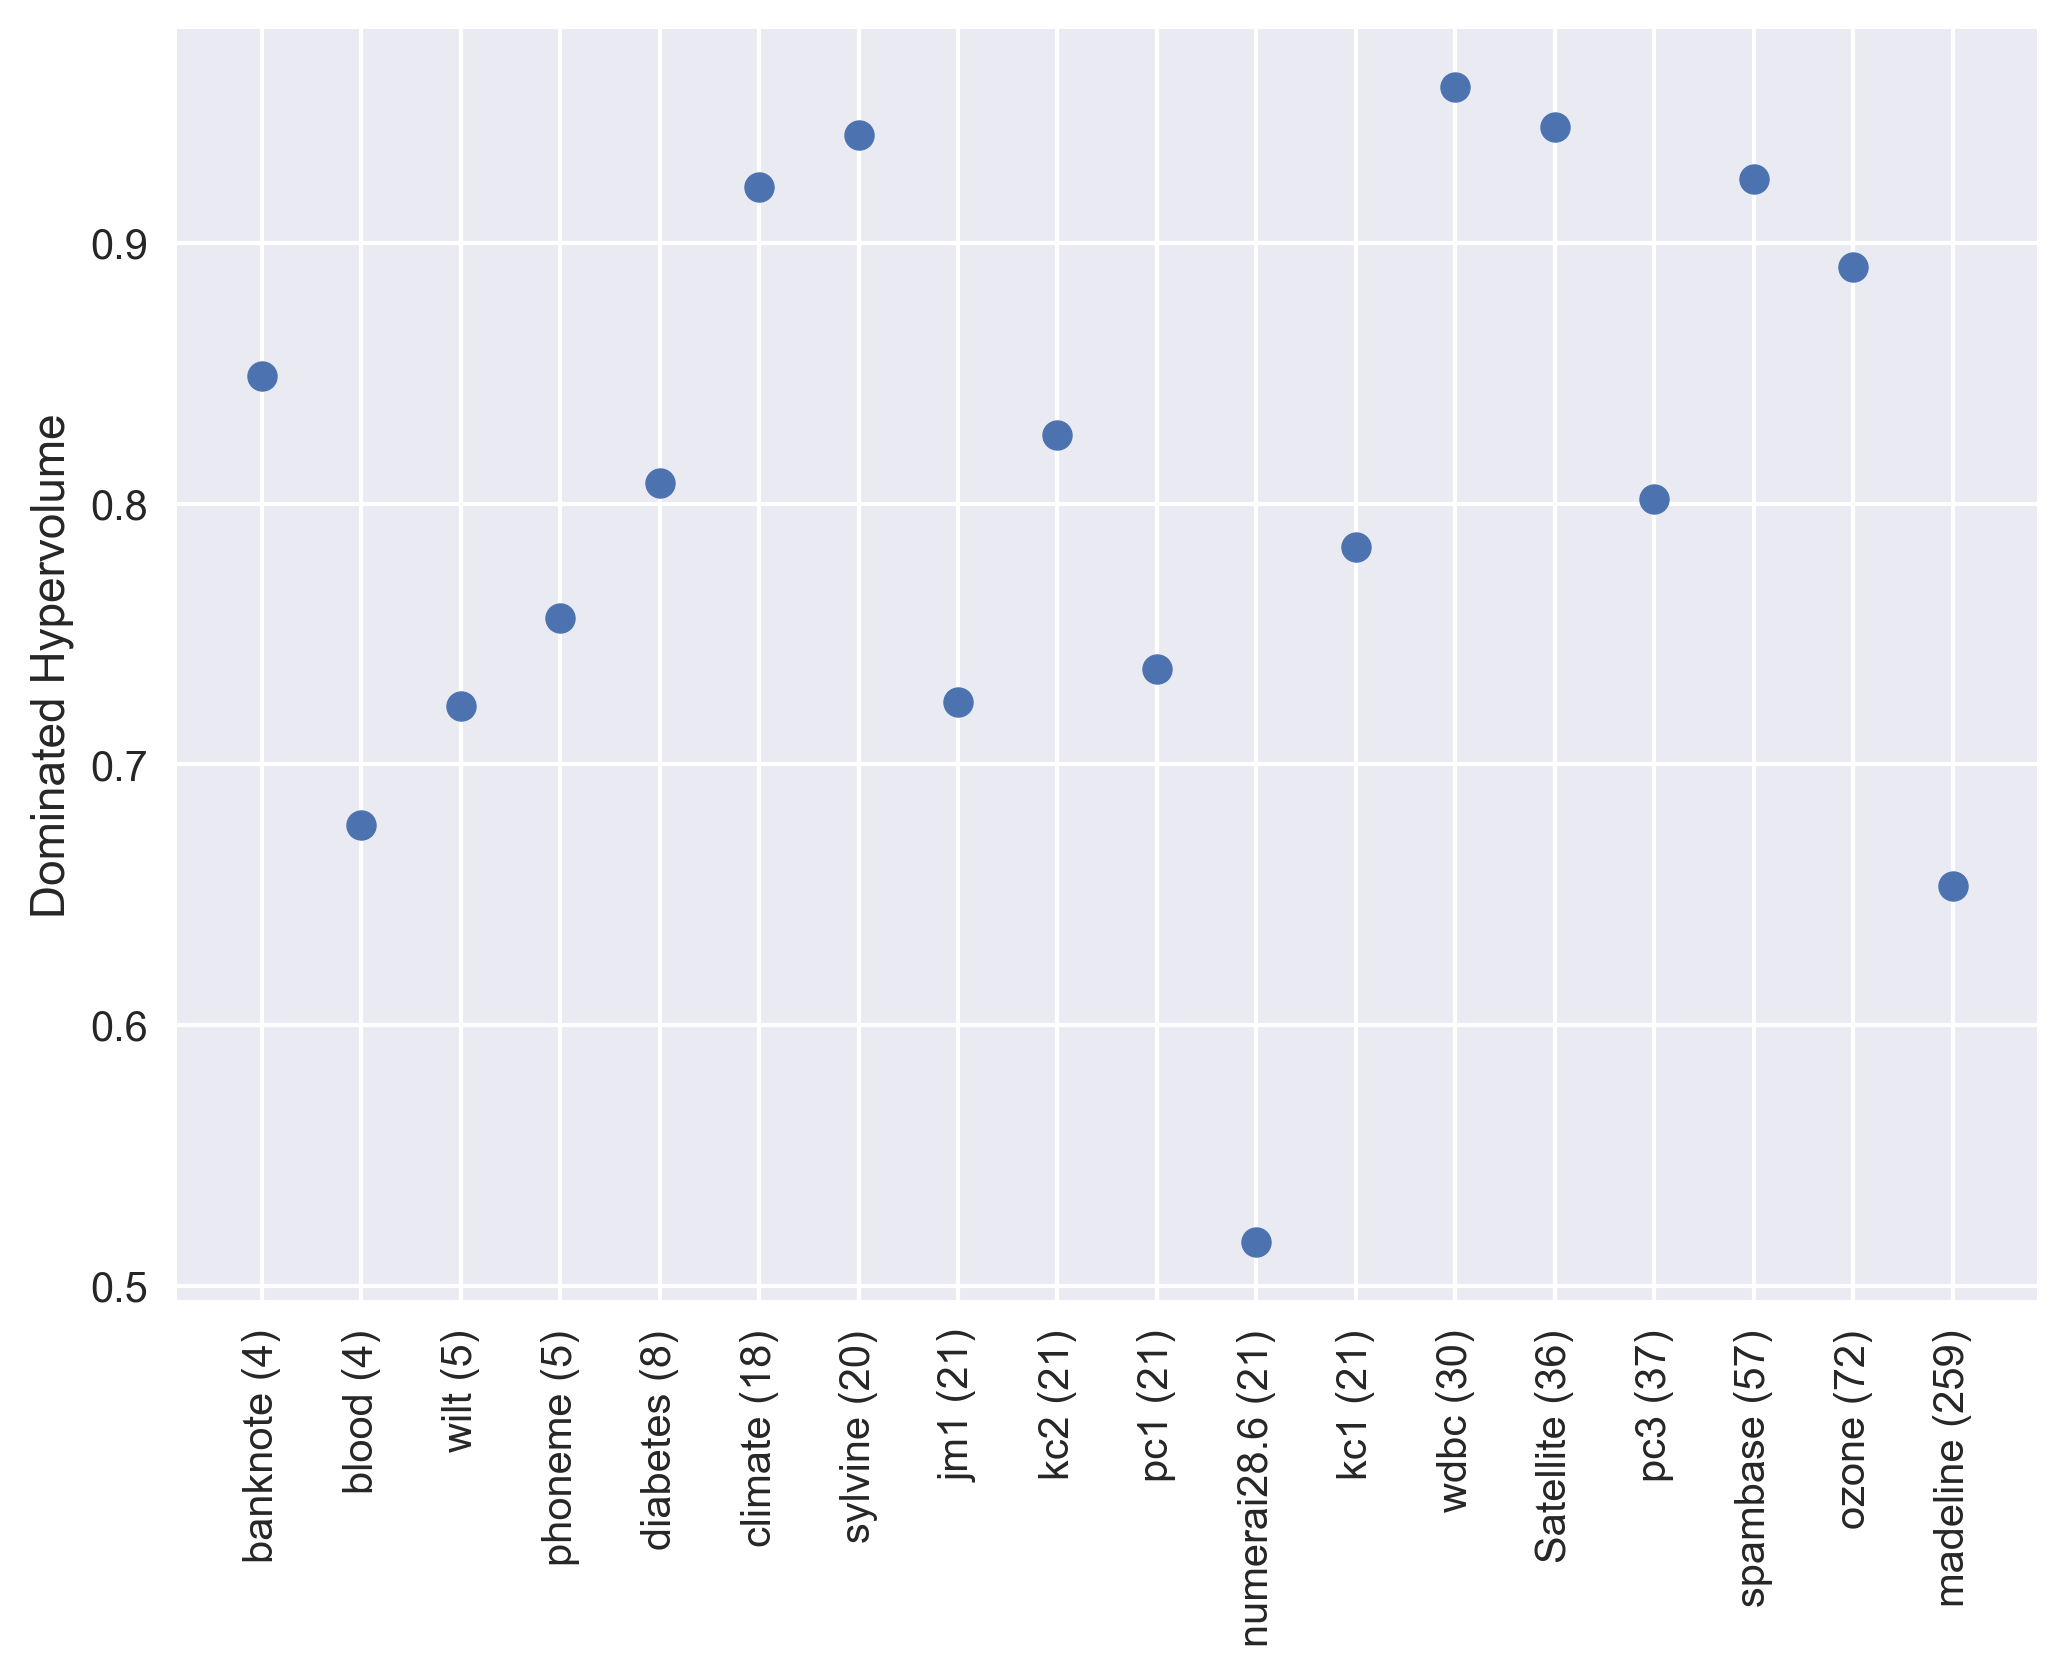
\includegraphics[width=0.9\linewidth]{../code/export/plot_test_dhvs.png}
  \caption{TODO: caption}
  \label{fig-test-dhvs}
\end{figure}
- preliminary
  * our implementation of feature + interaction detectors likely tend to include  % belongs in "general algorithm"
    - more features + interactions for high p datasets
    - less for low p datasets
    - remember: original paper samples \# of features included from truncated geometric distribution, what is not mentioned is probability of this distribution
      is determined from fitting 10 trees + looking at relative \# of features used (cf. their github repo ~/R/TunerEAGGA.R function get\_n\_selected\_rpart())
    -> mlr3 default decision tree max depth 30
      * i.e. datasets with p < 30 might use all features, which translates to trunc geom prob = 1
      * vice-versa for p >> 30 datasets relative \# features < 0.5 (our trunc geom prob)
      * similar reasoning for pairwise interactions
  * individuals not in Pareto sets occassionally exhibit AUC < 0.5
    - this is not by mistake, usually AUC on binary target can simply be inverted (simply predict the opposite class)
    - for us this cannot easily be inverted due to monotonicity constraints (weights cannot simply be multiplied by -1 if constrained)
    - could happen e.g. due to AdamW and weight clipping (employed to enforce monotonicity)
      * AdamW uses momentum
      * possible scenario: large momentum would yield negative weights, but after epoch they're clipped to [0,infty) + training stops due to early stopping
      * weight clipping very imperfect way of enforcing monotonicity, but currently in pytorch unfortunately only way to implement this
- Figure \ref{fig-test-dhvs}
  * suggests comparable performance to XGBoost EAGGA
  * did not compare to unrestricted NN, would not be sensible, as NF, NI, NNM would be 1, hence hypervolume = 0, as values along 3 dimensions would be at reference point
  * as XGBoost EAGGA, NN EAGGA consistently outperforms union of competitors as evident from \citep[Figure 2]{EAGGA}
  * unfortunately due to time constraints no own union comparison with NN instead of XGBoost
- overview over pareto sets can be accessed on our github repo at ~/code/export/*.csv
  * NN HPs
    - total layers mostly 3-4, most commonly 3, goes as high as 7 (Satellite (36), diabetes (8))
    - nodes per hidden layer mostly 3-6, goes as high as 12 (diabetes (8))
    - p dropout goes as high as 0.7 (climate (18), spambase (57)), but mostly in the 0.1 to 0.3 range
  * group structures
    - great diversity in NF across datasets
      * phoneme (5) up to 1
      * blood (4) up to 1
      * banknote (4) up to 0.75
      * diabetes (8) up to 0.5
      * climate (18) up to 0.67
      -> low p datasets in the benchmark tend to have higher NF
        - possible consequence of shorter evaluation time
        - low p datasets have much higher \# generations
        - group structure space much more likely to be exhausted, i.e. more exploration of NN hps
    - NI, NNM consequently (bounded by NF, can never be more than max \# for respective \# included features) rather low
  * dhv contributions
    % TODO: put explanation in line 400, don't introduce new topic here
    - measures contribution of an individual to the hypervolume, i.e. difference between hypervolume of entire pareto front vs hypervolume of pareto front without
      individual $\boldsymbol\lambda$: $\text{CON}_{\mathcal{P}}(\boldsymbol\lambda)=\text{HYP}(\mathcal{P})-\text{HYP}(\mathcal{P}\setminus\{\boldsymbol\lambda\})$,
      where $\text{HYP}(\mathcal{P})$ denotes the hypervolume induced by the pareto set $\mathcal{P}$ \citep[p. 384]{10.5555/1943267.1943271}
    - predominately low for fitted models
    - mostly highest for featureless learner predicting majority class
    -> sign of good exploration of pareto front + stable estimate, refer Section \ref{sec-moo-post}
- loss graphs Figure \ref{fig-es-losses}
  * suggests models could have benefitted from longer training on some datasets, as some loss curves haven't converged when stopping criterion hit
  * crit was likely triggered by short-term spike, thus could potentially be resolved by comparing average of last k losses against average of >patience< losses prior
    to that to not be as exposed to short-term spikes in loss
  * on other datasets, graphs suggest earlier stop would have been totally fine as the networks have long converged, but longer training likely not an issue as loss
    graphs come from early stopping dataset portion, which is disjunct from training set
- dhv over generations Figure \ref{fig-val-dhvs}
  * compute on val set, i.e. had 5 folds per individual
    - NF, NI, NNM always the same for each fold
    - but 5 different AUCs
    -> hypervolume of (mean(AUC 1, AUC 2, ..., AUC 5), NF, NI, NNM)
  * artifacts / drops along y likely due to inconsistent computation of Pareto front by third-party library
    - preliminary experiments on dummy pareto fronts with 10x4 metrics: noticed nds function returning different rankings for same front
    - returned ranking switched back and forth between two only slightly different options (only 1 or 2 indices were swapped)
    - not sure what caused this, as made same observation using another library that was planned as alternative
    - thus unfortunately not fixable for me
  * all but 3 datasets (2 of which only trained for 1 generation, aynway) show improvement of dominated hypervolume over generations
  * BUT: absolute as well as relative improvement almost negligible -> no large final dhv decrease would we just have evaluated the models gotten from the detectors
    - this was also the reason we didn't run EAGGA on philippine and gina simply without the detectors (as that's where they crashed) -> evidence suggested that detectors are vital to initial performance
    - original paper supports this assumption \citep[Fig. 4, p. 545]{EAGGA}


\section{Conclusion and Future Outlook}
(Conclusion)
- tabular data still difficult discipline for neural networks
- research suggests heavy regularisation to improve performance on tabular data
- EAGGA proved to be successful in making XGBoost more interpretable while keeping performance on par with unregularised XGBoost
- we extend EAGGA to neural networks to see if we can utilise the regularisation induced by it to make NNs both interpretable and performant on tabular data
- as consequence propose new architecture allowing to model equivalence relations of EAGGA
- ... conforming to \citet[chap. 2]{survey_NN_interpretability} taxonomy it fits as ..., ..., ... %TODO
- found overall performance comparable to that of XGBoost fitted using EAGGA, which is a plus, but no outperformance

(Future Outlook)
- MO BO on group structure space possible, perhaps via restricted BO?

% Manual newpage inserted to improve layout of sample file - not
% needed in general before appendices/bibliography.

%\newpage  % we are not to add page breaks


\vskip 0.2in
\bibliography{references}


\appendix
\section{Software used}
for implementation we used
openml \cite{OpenML}, \cite{OpenMLPython},
numpy \cite{numpy},
pandas \cite{pandas1}, \cite{pandas2},
pytorch \cite{PyTorch},
scikit-learn \cite{scikit-learn},
scipy \cite{SciPy},
pymoo \cite{pymoo}, and
tqdm \cite{tqdm}

\section{Plots}
\begin{figure}
  \centering
  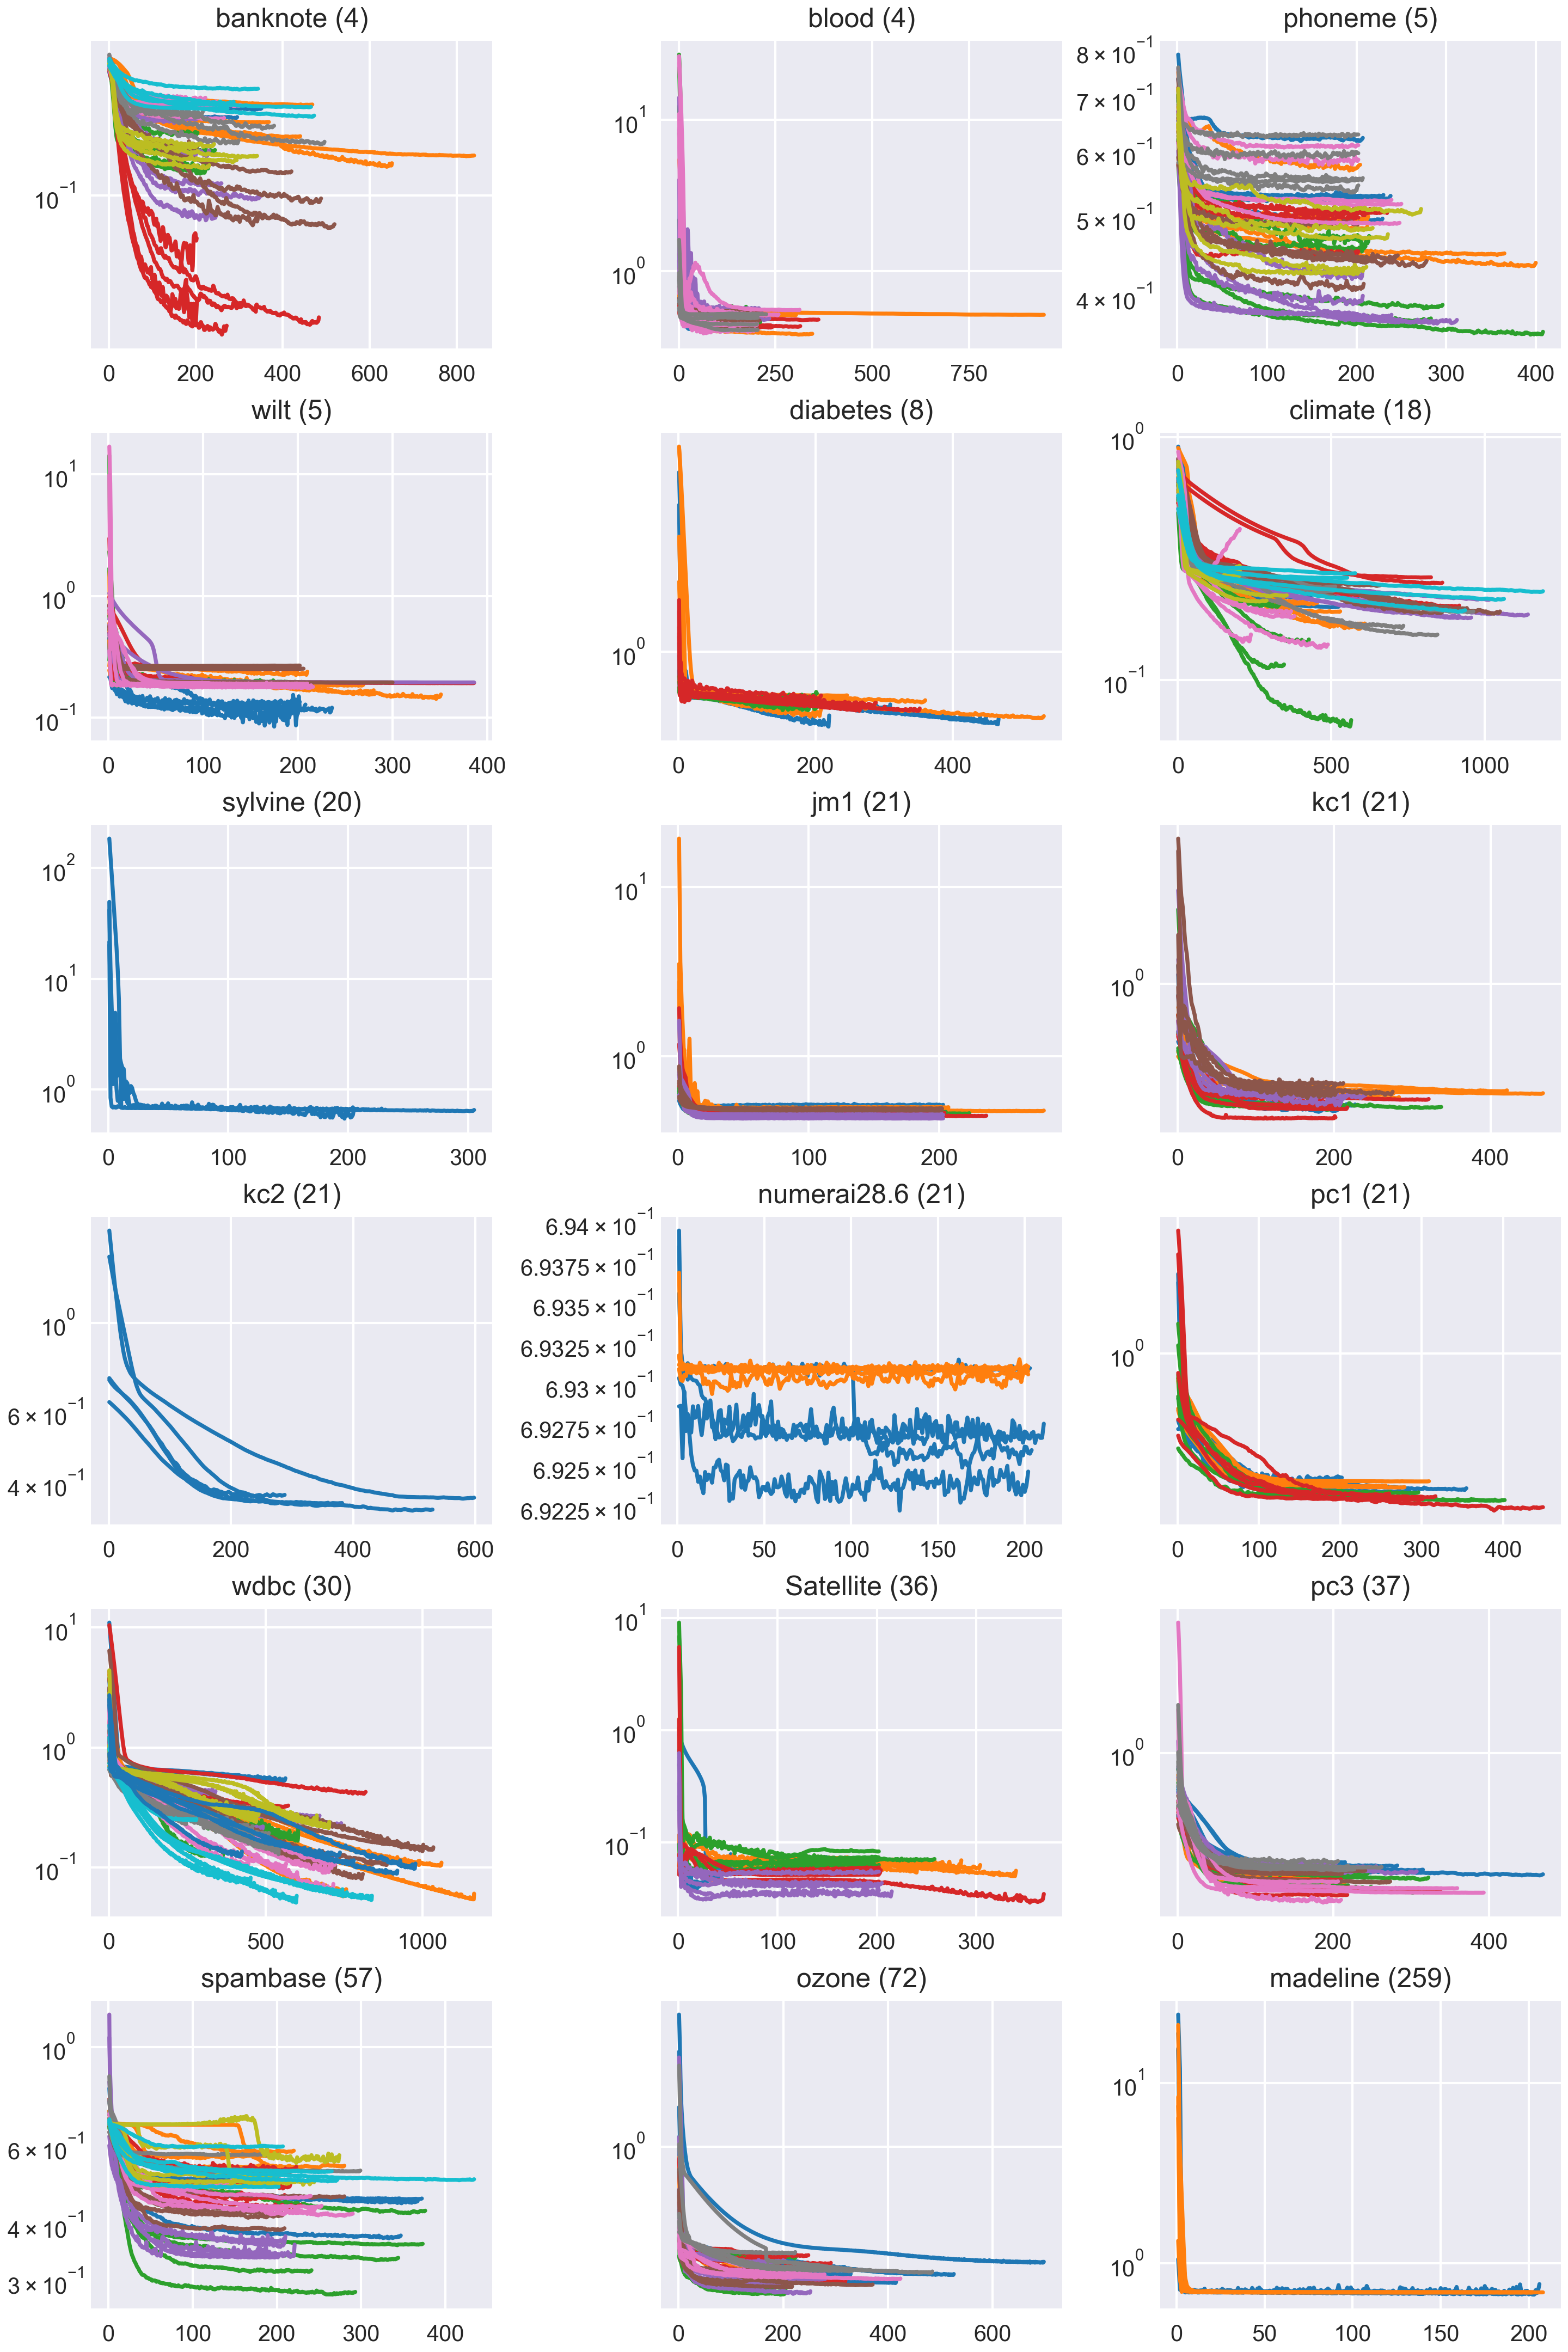
\includegraphics[width=0.9\linewidth]{../code/export/plot_early_stopping_losses_pareto_set.png}
  \caption{Pareto set loss of all datasets, evaluated on early stopping set. Same colours denote losses coming from folds of the same individual.
            x-axis portrait epochs, y-axis binary cross entropy loss.}
  \label{fig-es-losses}
\end{figure}

\begin{figure}
  \centering
  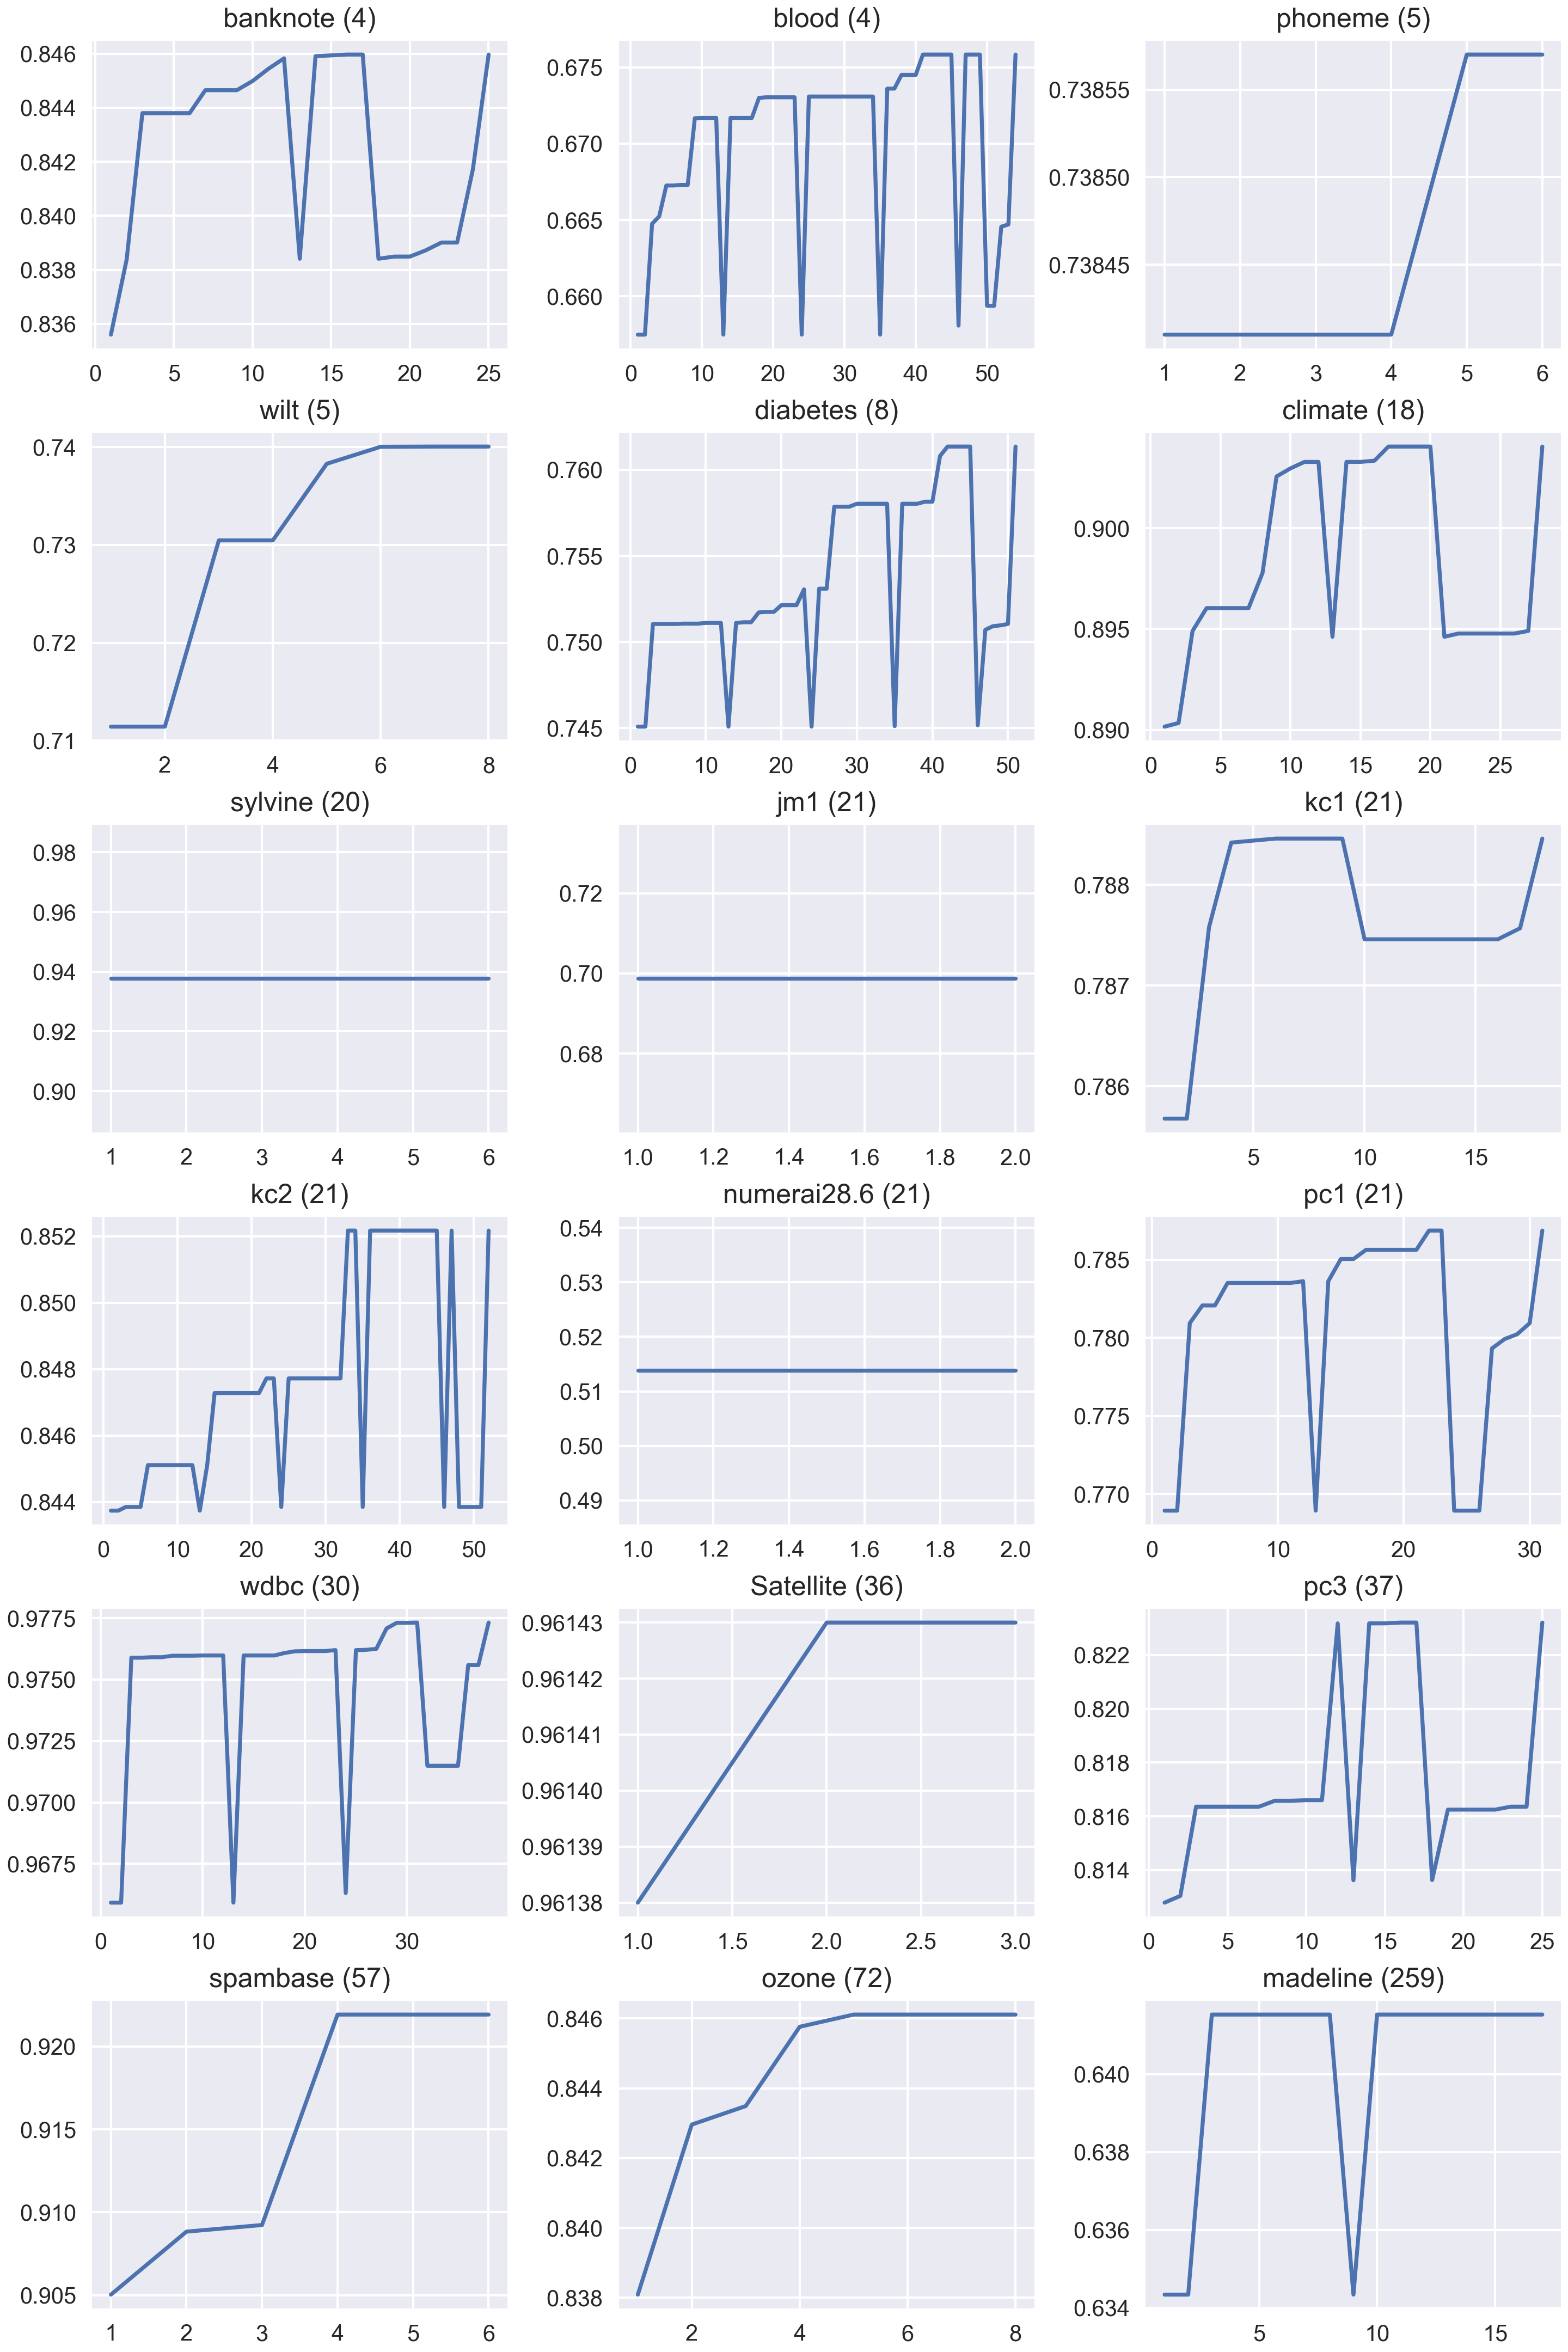
\includegraphics[width=0.9\linewidth]{../code/export/plot_val_dhvs_over_time.png}
  \caption{Dominated hypervolume over generations, evaluated on validation set.
            x-axis portrait generations, y-axis dominated hypervolume using mean AUC over folds.}
  \label{fig-val-dhvs}
\end{figure}

\end{document}
